Some public domain datasets were used in this FYP while learning TensorFlow and conducting empirical studies.
These datasets are outlined below.
\tocless\subsection{Food-101}
\parencite{food101} created the Food-101 dataset which consists of 101 different food types.
Each food type in the dataset has 1,000 images associated.
These images can be divided up into a training, test and validation set as seen fit by the user.
The Food-101 dataset is open for public use if it is used for research purposes and not for commercial use.
Examples from the Food-101 dataset can be seen in below.

\begin{figure}[h] 
  \label{food} 
  \begin{minipage}[b]{0.25\linewidth}
    \centering
    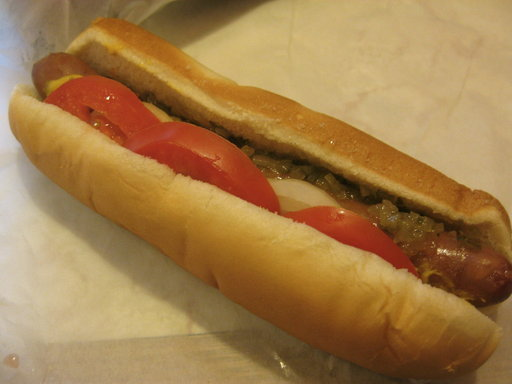
\includegraphics[width=.75\linewidth]{food1} 
    \caption{Hotdog} 
    \vspace{4ex}
  \end{minipage}%%
  \begin{minipage}[b]{0.25\linewidth}
    \centering
    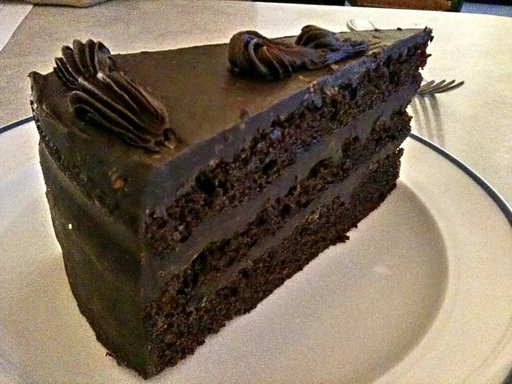
\includegraphics[width=.75\linewidth]{food2} 
    \caption{Chocolate Cake} 
  \label{fig:page2}
    \vspace{4ex}
  \end{minipage} 
  \begin{minipage}[b]{0.25\linewidth}
    \centering
    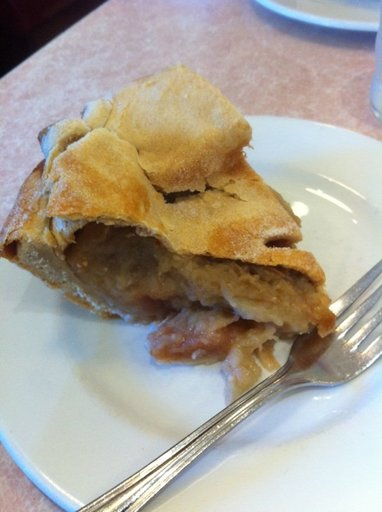
\includegraphics[width=.75\linewidth]{food3} 
    \caption{Apple Pie} 
    \vspace{4ex}
  \end{minipage}%% 
  \begin{minipage}[b]{0.25\linewidth}
    \centering
    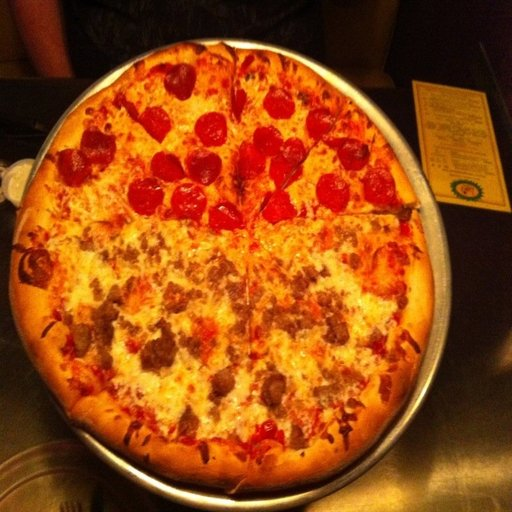
\includegraphics[width=.75\linewidth]{food4} 
    \caption{Pizza} 
    \vspace{4ex}
  \end{minipage} 
\end{figure}

\tocless\subsection{MNIST}
The MNIST dataset (created by \parencite{mnist}) consists of 70,000 hand written digits.
It is widely used in introductory CNN tutorials.
The dataset is split into 60,000 training images and 10,000 test images.
All the images are of the same dimensions.
Examples from the MNIST dataset can be seen in below.

\begin{figure}[h] 
  \label{mnistDataset} 
  \begin{minipage}[b]{0.25\linewidth}
    \centering
    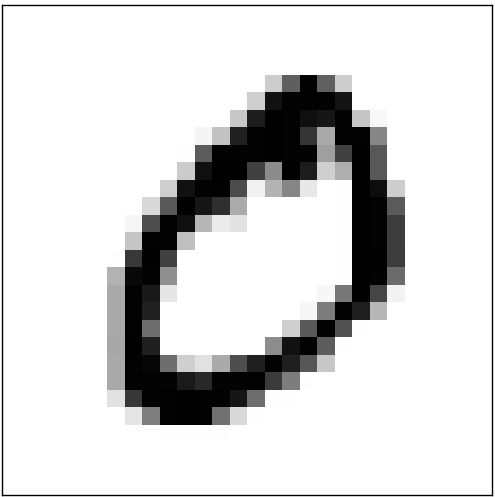
\includegraphics[width=.75\linewidth]{mnist0} 
    \caption{MNIST 0} 
    \vspace{4ex}
  \end{minipage}%%
  \begin{minipage}[b]{0.25\linewidth}
    \centering
    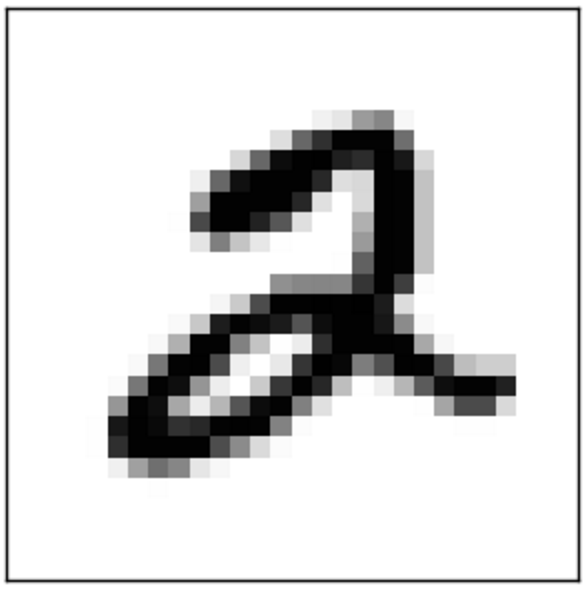
\includegraphics[width=.75\linewidth]{mnist2} 
    \caption{MNIST 2} 
  \label{fig:page2}
    \vspace{4ex}
  \end{minipage} 
  \begin{minipage}[b]{0.25\linewidth}
    \centering
    
\includegraphics[width=.75\linewidth]{mnist4} 
    \caption{MNIST 4} 
    \vspace{4ex}
  \end{minipage}%% 
  \begin{minipage}[b]{0.25\linewidth}
    \centering
    
\includegraphics[width=.75\linewidth]{mnist5} 
    \caption{MNIST 5} 
    \vspace{4ex}
  \end{minipage} 
\end{figure}

\tocless\subsection{CIFAR-10}
\parencite{cifar} created the CIFAR-10 dataset which consists of 10 classes.
Each of the 10 classes has 6,000 32x32 colour image associated and these are split between a 5,000 image training set and a 1,000 image test set.
There are five training batches and one test batch in the dataset.
The test set contains 1,000 randomly selected images from each class.
The training batches consist of random orderings of the remaining images.
Examples from the CIFAR-10 dataset can be seen below.

\begin{figure}[h] 
  \label{cifar10} 
  \begin{minipage}[b]{0.25\linewidth}
    \centering
    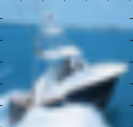
\includegraphics[width=.75\linewidth]{cifar1} 
    \caption{CIFAR-10 Truck} 
    \vspace{4ex}
  \end{minipage}%%
  \begin{minipage}[b]{0.25\linewidth}
    \centering
    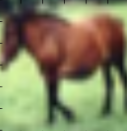
\includegraphics[width=.75\linewidth]{cifar2} 
    \caption{CIFAR-10 Horse} 
  \label{fig:page2}
    \vspace{4ex}
  \end{minipage} 
  \begin{minipage}[b]{0.25\linewidth}
    \centering
    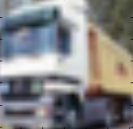
\includegraphics[width=.75\linewidth]{cifar3} 
    \caption{CIFAR-10 Boat} 
    \vspace{4ex}
  \end{minipage}%% 
  \begin{minipage}[b]{0.25\linewidth}
    \centering
    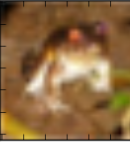
\includegraphics[width=.75\linewidth]{cifar4} 
    \caption{CIFAR-10 Frog} 
    \vspace{4ex}
  \end{minipage} 
\end{figure}